\index{Desarrollo|(}
\section{Desarrollo}

\subsection{Implementaci\'on de Matriz:}

Era a libre elecci\'on decidir como implementar la matriz, una manera eficiente nos pareci\'o usar punteros a punteros para almacenar los valores de A. Como tenemos un conjunto acotado de valores que no son cero(Banda p,q), por cada fila nos quedamos con los p+q+1 que nos interesan. Sobre el resto de las funciones no queda mucho mas que decir, ya que no presentaron problemas en su implementaci\'on. El c\'odigo se ejecuta, pasando por par\'ametro h,n,span, los valores que son dato C1..Cn-1, el costo C, y la fuerza m\'axima l\'imite, en el archivo ayuda.txt se explica mas detalladamente el orden de los par\'ametros y ejemplos de su uso.\newline
Mediante el uso de memoria din\'amica conseguimos que luego en la experimentaci\'on se pueda hacer libremente sin tener que estar resguard\'andonos de estar usando demasiada memoria; Fuimos capaces de experimentar con puentes de gran tama\~{n}o.

\subsection{Realizacion del TP:}

El problema a resolver en el TP, era el de representar un puente Pratt Trauss, estable, en un sistema de ecuaciones, la complejidad que presentaba esto, constaba de distintas cuestiones:

\begin{itemize}
\item[1] En principio, como organizar las partes del puente, los links y juntas, para que nos quede un sistema de ecuaciones y de ah\'i poder despejar las fuerzas que ejerc\'ia cada link, dada la cantidad de juntas, y otros datos como el span y la altura.El problema presentado nos indicaba que esto iba a ser posible armando la matriz de $4n$x$4n$, el vector de inc\'ognitas era justo de $4n$ y a partir de las relaciones f\'isicas de las distintas fuerzas un vector b de, tambi\'en, $4$x$n$, entonces se consegu\'ia un sistema estable Ax=b.\newline
Los vectores x y b, eran pr\'acticamente datos del input, la matriz A era un poco mas complicada de construír, o por lo menos, fue necesario ordenar las fuerza, de forma tal que quede un sistema conveniente, una matriz banda. El orden de las fuerzas es f\'acil de explicar mediante un ejemplo:\newline

\begin{figure}[!ht]
\begin{center}
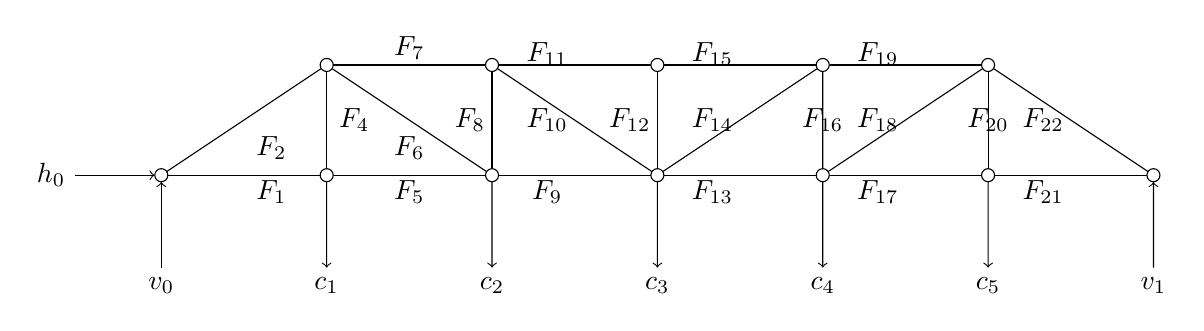
\begin{tikzpicture}[scale = 0.7]

    \tikzset{nodestyle/.style={draw,shape=circle,scale=0.5}}
    \node[nodestyle] (p1) at ( 0, 0) {};
    \node[nodestyle] (p2) at ( 3, 0) {};
    \node[nodestyle] (p3) at ( 6, 0) {};
    \node[nodestyle] (p4) at ( 9, 0) {};
    \node[nodestyle] (p5) at ( 12, 0) {};
    \node[nodestyle] (p6) at ( 15, 0) {};
    \node[nodestyle] (p7) at ( 18, 0) {};

    \node[nodestyle] (p8) at ( 3, 2) {};
    \node[nodestyle] (p9) at ( 6, 2) {};
    \node[nodestyle] (p10) at ( 9, 2) {};
    \node[nodestyle] (p11) at ( 12, 2) {};
    \node[nodestyle] (p12) at ( 15, 2) {};

    \begin{scope}[every path/.style={-}]
        \draw (p1) -- (p2);
        \draw (p2) -- (p3);
        \draw (p3) -- (p4);
        \draw (p4) -- (p5);
        \draw (p5) -- (p6);
        \draw (p6) -- (p7);

        \draw (p8) -- (p9);
        \draw (p9) -- (p10);
        \draw (p10) -- (p11);
        \draw (p11) -- (p12);

        \draw (p1) -- (p8);
        \draw (p12) -- (p7);

        \draw (p2) -- (p8);
        \draw (p3) -- (p9);
        \draw (p4) -- (p10);
        \draw (p5) -- (p11);
        \draw (p6) -- (p12);

        \draw (p8) -- (p3);
        \draw (p9) -- (p4);
        \draw (p4) -- (p11);
        \draw (p5) -- (p12);
    \end{scope}

    
    \node (v0) at ( 0, -2) {$v_0$};
    \node (v1) at ( 18, -2) {$v_1$};
    \node (h0) at ( -2, 0) {$h_0$};
    \node (c1) at ( 3, -2) {$c_1$};
    \node (c2) at ( 6, -2) {$c_2$};
    \node (c3) at ( 9, -2) {$c_3$};
    \node (c4) at ( 12, -2) {$c_4$};
    \node (c5) at ( 15, -2) {$c_5$};

    \node (f1) at ( 2, -0.3) {$F_1$};
    \node (f2) at ( 2, 0.5) {$F_2$};
    \node (f4) at ( 3.5, 1) {$F_4$};
    \node (f5) at ( 4.5, -0.3) {$F_5$};
    \node (f6) at ( 4.5, 0.5) {$F_6$};
    \node (f7) at ( 4.5, 2.3) {$F_7$};
    \node (f8) at ( 5.6, 1) {$F_8$};
    \node (f12) at ( 8.5, 1) {$F_{12}$};
    \node (f16) at ( 12, 1) {$F_{16}$};
    \node (f20) at ( 15, 1) {$F_{20}$};
    \node (f9) at ( 7, -0.3) {$F_9$};
    \node (f10) at ( 7, 1) {$F_{10}$};
    \node (f11) at ( 10, 1) {$F_{14}$};
    \node (f12) at ( 13, 1) {$F_{18}$};
    \node (f22) at ( 16, 1) {$F_{22}$};

    \node (f11) at ( 7, 2.2) {$F_{11}$};
    \node (f15) at ( 10, 2.2) {$F_{15}$};
    \node (f19) at ( 13, 2.2) {$F_{19}$};
    \node (f13) at ( 10, -0.3) {$F_{13}$};
    \node (f17) at ( 13, -0.3) {$F_{17}$};
    \node (f21) at ( 16, -0.3) {$F_{21}$};


    %\begin{scope}[every path/.style={-}]
        \draw[->] (v0) -- (p1);
        \draw[->] (v1) -- (p7);
        \draw[->] (h0) -- (p1);
        \draw[->] (p2) -- (c1);
        \draw[->] (p3) -- (c2);
        \draw[->] (p4) -- (c3);
        \draw[->] (p5) -- (c4);
        \draw[->] (p6) -- (c5);
    %\end{scope}

        % Nodos artificiales.
         
\end{tikzpicture}
\caption{Fuerzas aplicadas sobre la estructura}
\label{fig:structload}
\end{center}
\end{figure}

Este orden es conveniente porque al tomar las filas de A como las ecuaciones de fuerzas horizontales y verticales queda una matriz banda, con p,q acotable a un valor fijo no muy grande. En nuestra implementaci\'on con p,q = 6 obtuvimos buenos resultados.


\item[2] Una vez que conseguimos $Ax=b$, un algoritmo hace la factorizaci\'on PLU de A, mediante Eliminaci\'on Gaussiana con pivoteo parcial, y con forward y backward substitution obtenemos el $x$ con los resultados de las fuerzas. Un dato a tomar en cuenta es que en la implementaci\'on de la matriz, a pesar de ser eficientes, los arreglos de valores distintos de cero complican hacer el cambio de filas que requiere el pivoteo, para eso nos dimos la libertad de usar un poco mas de memoria dinamica para asegurarnos que no se indefina en algunos casos.(CAMBIABLE)

\item[3] La segunda parte del TP, el agregado de pilares, lo resolvimos haciendo que el algoritmo vea que ocurre si se inserta un pilar en donde tenemos la fuerza m\'axima, de ah\'i en los dos bloques que quedan se eval\'ua si las fuerzas m\'aximas de ellos es mayor o no a la fuerza m\'axima anterior, si se consigue disminuir, la inserci\'on es conveniente, y de ah\'i se sigue analizando recursivamente en las 2 estructuras hasta conseguir fuerzas m\'aximas menores al parámetro FMAX.\newline

\end{itemize}

\subsection{Hip\'otesis:}

\begin{itemize}

\item Variando Span: Al variar este par\'ametro se logra que los links horizontales se agranden y los links colocados como una hipotenusa tambien aumentan su tama\~{n}o, creemos que al ocurrir esto el puente ser\'a m\'as inestable, osea que va a resistir fuerzas m\'as d\'ebiles.

\item Variando n: Podemos ver que gracias a este par\'ametro cambia la cantidad de $C_i$ y por lo tanto podemos notar que los dem\'as links quedar\'an tirantes produciendo que el link haga m\'as fuerza que antes si este valor aumenta.

\item Variando h: Al variar este par\'ametro obtenemos m\'as altura de la estructura, aumenta el tama~{n}o de los links verticales. Y por lo tanto tambien modifica los links colocados de forma hipotenusa. Esto produce modificaciones y analizaremos si podemos conseguir mejorar costos y fuerzas al tomar diferentes valores.

\item Variando $C_i$: Variando este par\'ametro se consigue tener mas o menos cantidad de fuerza ejercida sobre cada una de las juntas que posee n. Esto puede ocasion variaciones en las fuerzas y por lo tanto analizaremos como se efectuan estos cambios.

\item Variando $F_{MAX}$: Si bien el variar este par\'ametro no presenta muchas cosas interesantes para analizar, hemos realizado experimentaciones para ver exactamente como varia la inserci\'on de pilares con este valor, ya que se ve a simple viste q disminuyendolo aumentara la cantidad de inserci\'on de pilares y aumentandolo disminuir\'a la cantidad de pilares.

\end{itemize}

\subsection{Experimentacion:}

\begin{itemize}
\item[1] En vista de lo mencionado en la seccion hip\'otesis, hemos optado por experimentar dejando un valor fijo y variando los otros para ver como afecta en los resultados.

\item[2] Para las experimentaciones hemos optado por der el mismo valor a todos los Ci y ver como var\'ia al aumentar proporcionalmente de la misma forma cada uno.

\item[3] Hemos optado por realizar lo comentado en el enunciado, analizar como vari\'an las fuerzas m\'aximas y luego ver como var\'ian los costos (se observar\'a en los resultados las dos secciones separadas).

\end{itemize}

\index{Desarrollo|)}